\chapter{Zebrafish Analysis}\label{chap:results}

This chapter is divided into three sections. First section presents result related to ISV analysis. We will compare proposed automated segmentation of ISV against manual segmentation. Further to identify whether chemicals from ToxCast Phase I library are vascular disruptor compounds, we present how ISV features can be used to discriminate healthy embryo from abnromal embryos. ISV features are used to train a linear classifier for depicting embryos impacted with toxicity. 

Second section will focus on CVP analysis, presenting classification results using GLCM, HOG, Co-HOG, and proposed gCo-HOG. In third section, we will explore the relationship between increasing dosage of chemicals with impact on ISV, and CVP separately. We will discuss how many chemicals impacted ISV and CVP or both.

Last section will present results showing variations in temporal growth of embryo for healthy against treated. 


\section{Intersegmental Vessel Analysis}\label{sec:isvanalysis}
ISV results are presented for entire zebrafish vasculature recorded from the fluorescence microscope. 

\subsection{Segmentation Analysis}
Segmentation of ISV can be a time consuming process. ISVs occur in various size and shows huge variation in intensity. Method in section \ref{sec:isvseg} to segment the ISV from zebrafish images. The accuracy of the automatic segmentation of ISVs is determined by the comparisons between manual segmentation and the automated. 30 randomly chosen ISVs are manually segmented in the RGB color space, and compared. Vessels are visually inspected by two users (fig. \ref{isvseg}). 


Accuracy, Precision and recall measures and F-score are used to define error \cite{Martin01}. The error measures used are defined as follows:
\begin{equation}
Accuracy = \frac{tp + tn}{(tp + tn + fp + fn)}
\end{equation}

\begin{equation}
Precision = \frac{tp}{(tp + fp)}
\end{equation}

\begin{equation}
Recall = \frac{tp}{(tp + fn)}
\end{equation}

\begin{equation}
F - score = 2*\frac{(Precision * Recall)}{(Precision + Recall)}
\end{equation}

 \begin{figure}[H] 
 \begin{center}
    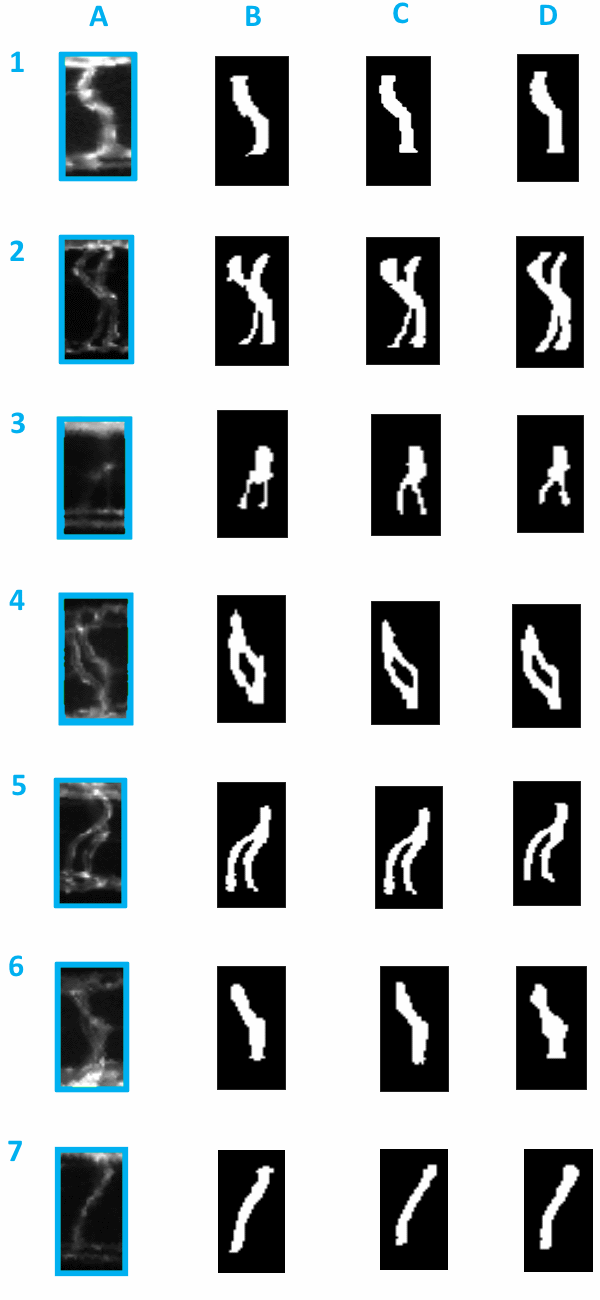
\includegraphics[scale=0.5]{figure/isvSegmentation.png}
  \end{center}
  \caption[ISV segmented images]{Comparison between automated segmentation and manual segmentation by user1 and user 2 of zebrafish embryos. (A) Analyzed ISV (B) Automated segmentation (C) User 1 segmentation (D) User 2 segmentation}
 \label{isvseg}
\end{figure}


where tp is the number of true positives, tn is the true negatives count, fp is the number of false positives and fn is the number of false negatives. The output of the segmentation is a binary vector with the same size as the image. A true positive is when output of
our segmentation is 1 when manual users marked it as 1, a true negative is when the output of the segmentation is 0 while the manual users labeled it as 0, a false positive is when the output of the segmentation is 1 when users label is 0, and a false negative is when the output of the segmentation is 0 while the users label is 1. We used the above mentioned error to quantitate how close the automated method is to manual segmentation. We have shown the results for 30 randomly chosen zebrafish ISVs by two users in fig. \ref{segResult}. 


\begin{table}[htb] 
\begin{center}
	\caption{Segmentation results for ISV} 
	
    \begin{tabular}{| c | c | c |}
    \hline\hline
    \textbf{Analysis} & \textbf{User 1}  & \textbf{User 2} \\ \hline \hline
		Precision & 0.847 & 0.839  \\ \hline
		Recall & 0.826 & 0.828  \\ \hline
		Accuracy & 0.952 & 0.951  \\ \hline
		F - score & 0.834 & 0.830  \\ \hline
    \end{tabular}
		\label{table:segRes} 
\end{center}
\end{table}

The average accuracy for the ISVs with manual users are $0.952$ and $0.951$. Average f-score for both users are 0.830 and 0.832. More detailed results are presented in table \ref{table:segRes}. These results indicate that the automated segmentation is comparable to that by manual segmentation. 


 \begin{figure}[H] \centering
 \begin{center}
    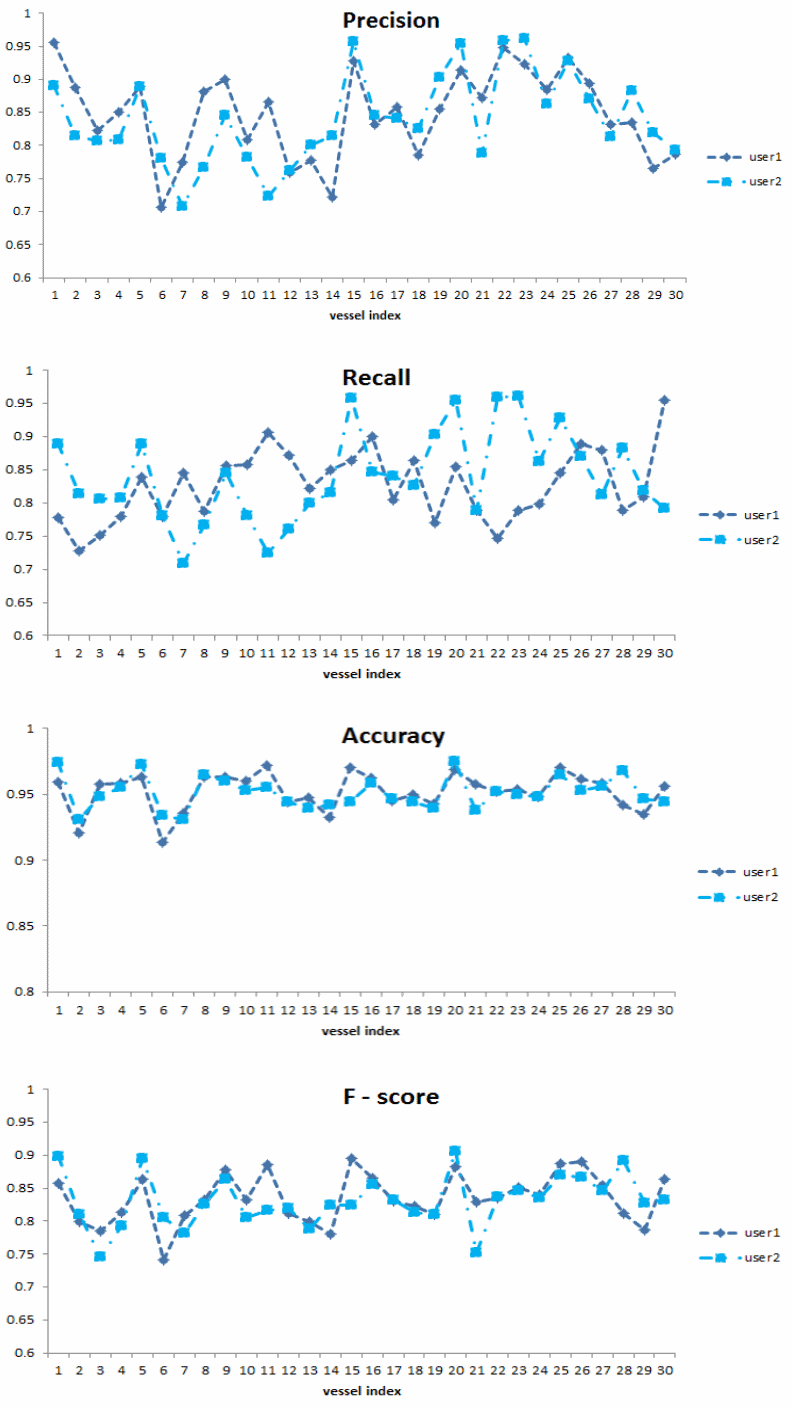
\includegraphics[scale=0.45]{figure/isvSegResult.png}
  \end{center}
  \caption[Comparison between the automated segmentation and manual segmentation of ISV.]{(a) Our approach have an average accuracy of 0.95 with user 1 and user 2. (b) Our approach have an average precision of 0.83 and 0.84 with with user 1 and user 2. (c) Average recall for both users is 0.83. (d) Lastly, average f - score for user are 0.83.}
 \label{segResult}
\end{figure}

\subsection{Toxicity impacts Intersegmental Vessels}

To identify whether chemicals from ToxCast Phase I library are vascular disruptor compounds (VDCs), 38 chemical are tested in a range of concentrations on zebrafish embryos from 3 hpf to 72 hpf in a single static exposure. Typically, the chemicals are tested from 100 nM to 20 $\mu$M. If the chemical exposures are lethal, lower and narrower dosages are tested. Visual analysis showed changes in ISV morphology due to chemical treatment. ISV abnormalities included the absence of ISV (fig. \ref{toxicity}), or thin and underdeveloped ISV (fig. \ref{toxicity}C). Quantitative image analysis is performed on the vascular disruption in the ISVs. 

\begin{figure}[H]\centering
  \begin{center}
    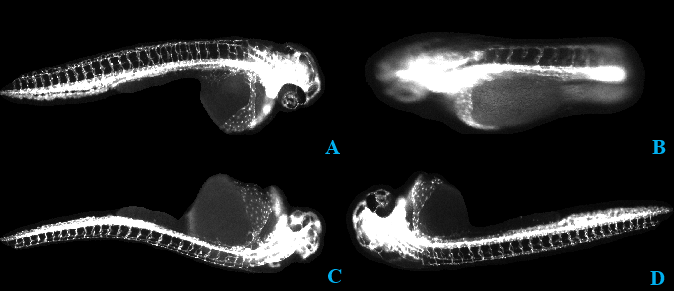
\includegraphics[scale=0.35]{figure/toxicityEffect.png}
  \end{center}
  \caption[Effect of toxins on ISV]{ Severity of toxins effect on zebrafish ISVs. High dosage can act as a ISV disruptor, and these effects can be quantified in terms of ISV count; average distance between ISV; total area of ISV; and an average ISV length. Figure \ref{toxicity}A shows an increment in ISV count, whereas \ref{toxicity}B shows decrement in ISV count.  Figure \ref{toxicity}C, \ref{toxicity}D embryos have small size ISV and occupy less area.}
  \label{toxicity}
\end{figure}


ISVs are first isolated from images using algorithm presented in section \ref{sec:isvseg} from the whole embryo and measured for ISV length, ISV distance, number of ISVs and ISV area. All terms are defined in pixels. We reported quantification results for 38 toxins. Previous research have shown the quantification terms used in this work can be used to analyze toxicity effect in ISV \cite{Feng05}, \cite{Tran07}, \cite{Vogt09}. Figure \ref{isvplots} shows with increasing toxins dosage, the ISV disruption becomes more prominent. Average ISV count, average distance between ISV, average ISV area and an average ISV length gradually decreases with increasing chemical dosage. %Details about an average ISV length, an average number of ISVs average ISV distance and an average ISV area are presented in table \ref{table:isvScreen}

To aid HTS of ISV for toxicity, we utilized features quantification to train a linear SVM classifier to identify zebrafish embryo with morphological changes. Dataset consists of 380 images of ISV. 190 images in the dataset did not show any abnormalities, while the remaining 190 images shows morphological changes to the ISV due to toxicity. Labels are visually obtained. We split the data into two parts. $1/3$ of data is used for parameter estimation for SVM and rest $2/3$ is used for training and testing. Parameters $(C, \gamma)$ are determined based on a grid-search that is conducted among $C$ $\epsilon$ ${2^{-10}, 2^{-4}, \cdots, 2^{10}}$ and $\gamma$ $\epsilon$ ${2^{-10}, 2^{-4}, \cdots, 2^{10}}$ with 3-fold cross-validation. Using the parameter values that achieved the best cross-validation accuracy, we then built a new model on the remaining data set, using 3-fold cross-validation. The optimal $C$ and $\gamma$ parameters are found to be 0.5 and 16, respectively, resulting in SVM model classification accuracy of $93.03\%$.

\begin{landscape}\centering
\begin{figure}[htb]
 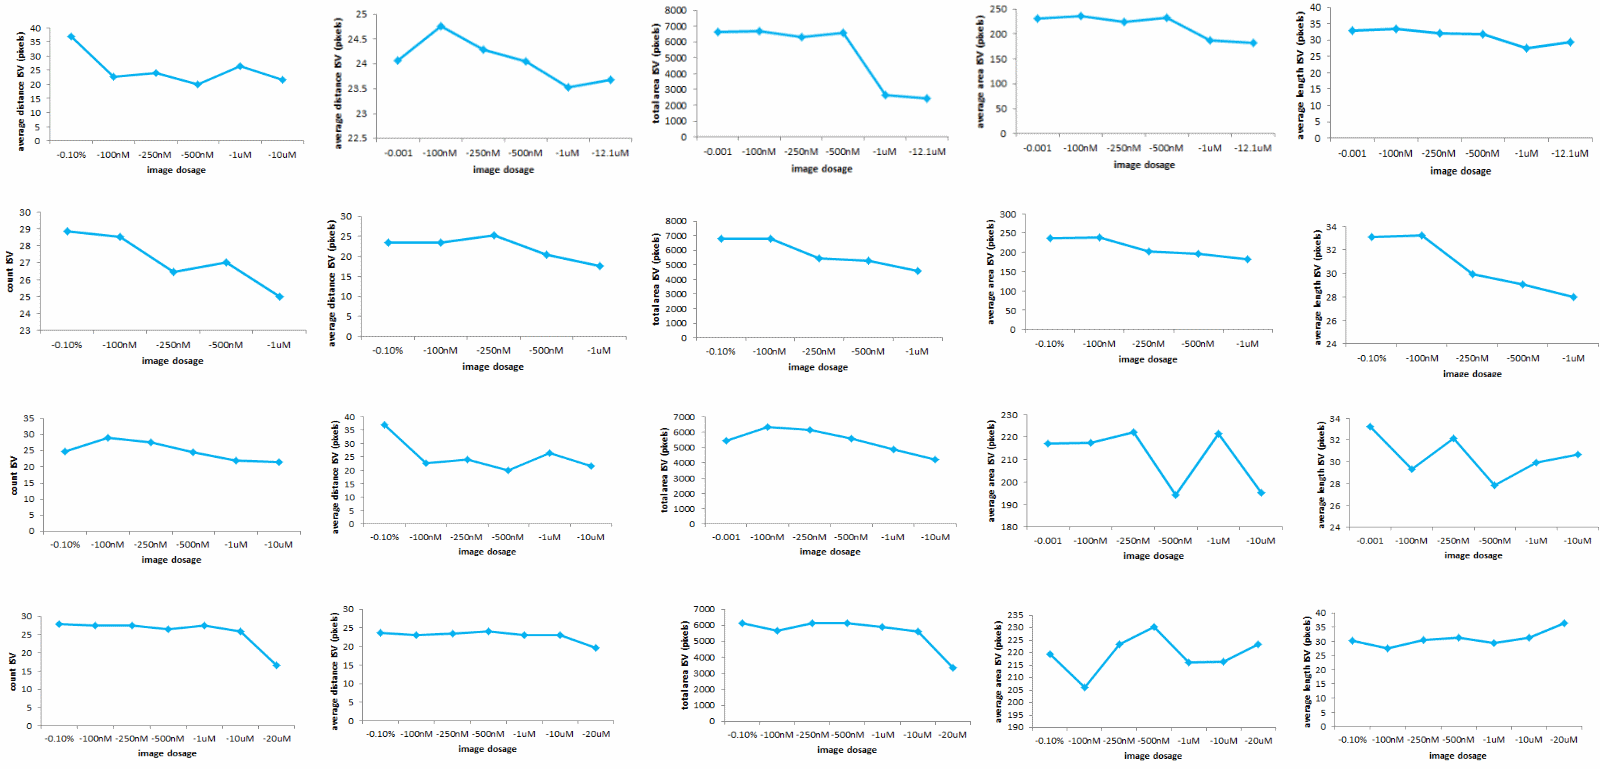
\includegraphics[scale=0.45]{figure/analysisPlot.png}
\caption[ Effect of toxins on ISV morphology]{Plots for various chemicals with variable dosage in comparison too untreated embryo (0.1\%). Each row corresponds to different chemicals. Within each row first plot shows variation in ISV count; Average ISV distance; Average ISV Area; Total SIV area;}\label{isvplots}
\end{figure}
\end{landscape}


\section{Toxicity impacts Caudal Vein Plexus}\label{sec:cvpanalysis}

CVP analysis results are presented for entire zebrafish vasculature recorded from the fluorescence microscope. We will present CVP analysis results using features explained in section \ref{sec:cvp}. We will empirically validate choice of parameters used for analysis. Dataset consists of 180 images of various size ($163 \times 55 - 331 \times 150$ pixels). 90 images in the dataset do not show any abnormalities, while the remaining 90 images show structural changes to the CVP due to toxicity effects (fig. \ref{cv} shows the images of healthy and treated zebrafish embryo). Labels are visually obtained. On similar lines ad CVP toxicity analysis We split the data into two parts. $1/3$ of data is used for parameter estimation and rest $2/3$ is used for training and testing. Parameters $(C, \gamma)$ are determined based on a grid-search that is conducted among $C$ $\epsilon$ {$2^{-10}, 2^{-4}, \cdot, 2^{10}$} and $\gamma$ $\epsilon$ {$2^{-10}, 2^{-4}, \cdot, 2^{10}$} with 3-fold cross-validation. Using the parameter values that achieved the best cross-validation accuracy, we then built a new model on the remaining data set, using 3-fold cross-validation. 

\begin{figure}[htb] \centering
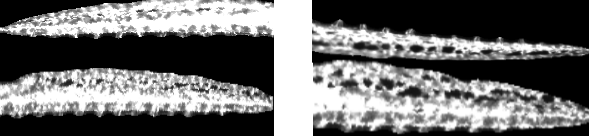
\includegraphics[scale=0.95]{figure/cv.png}
  \caption[Healthy and treated CVP]{Image on left shows healthy CVP and on right is the CVP observed for an embryo exposed to toxin. Loopy structure develops in CVP region for the treated embryo.}
 \label{cv}
\end{figure}

\subsection{Gray Level Co-occurrence Matrix Analysis}

Features energy, homogeneity, correlation, and contrast are calculated from each image using GLCM representing our image. We computed results with varying d ranging from 1-15. We obtain best results using d = 9. Table \ref{table:accglcm} shows comparison between accuracies with varying d. 

\begin{table}[h] 
\begin{center}
	\caption{Recognition results (\%) for GLCM with varying d} 
    \begin{tabular}{| c | c |}
    \hline
    \textbf{d} & \textbf{accuracy} \\  \hline \hline
		 1 & 73.02 \\  \hline
		 2 & 71.42 \\  \hline
		 3 & 80.15 \\  \hline
		 4 & 76.19 \\  \hline
		 5 & 76.91 \\  \hline
		 6 & 79.36\\  \hline
		 7 & 80.95 \\  \hline
		 8 & 76.98 \\  \hline
		 9 & 80.95 \\  \hline
		 11 & 75.39\\  \hline
		 12 & 80.74 \\  \hline
		 13 & 80.95 \\  \hline
		 14 & 78.57 \\  \hline
		 15 & 80.57 \\  \hline
    \end{tabular}
		\label{table:accglcm} 
\end{center}
\end{table}


The optimal $C$ and $\gamma$ parameters are found to be 65536 and 0.03, respectively, resulting in SVM model classification accuracy of $80.95\%$.

\subsection{Histogram of Gradient Analysis}
8 rectangular regions are tiled $M/4 \times N/2$ with no overlap. More tiles are made along the image width as CVP occupies more region along width as compared to height. To compare the effect of orientations, we generate histograms with orientation range from $[0, 360]$ and $[0, 180]$. Histograms with bin size $K$ ranging from 5 to 10 are evaluated. We got a best performance with bin size 6, 8, 9, 10 for $[0, 360]$ orientation (table \ref{table:acchog360} and \ref{table:acchog180}). We choose bin size of 6 and orientation range as $[0, 360]$. Thus the dimension of our feature is $(6 \times (4 \times 2)) = 1$. The optimal $C$ and $\gamma$ parameters are found to be 16 and 0.5, respectively.

\begin{table}[h] 
\begin{center}
	\caption{Recognition results (\%) for Co - HOG with varying bin size $K$ for $[0, 360]$ orientation} 
    \begin{tabular}{| c | c | c | c | c | c | c |}
    \hline
    \textbf{d} &  5  &  6  &  7  &  8  &  9  &  10\\  \hline
		 \textbf{accuracy} & 90.47 &  92.06  &  92.00  &  92.06  &  92.06  &  92.06 \\  \hline
    \end{tabular}
		\label{table:acchog360} 
\end{center}
\end{table}

\begin{table}[h] 
\begin{center}
	\caption{Recognition results (\%) for Co - HOG with varying bin size $K$ for $[0, 180]$ orientation} 
    \begin{tabular}{| c | c | c | c | c | c | c |}
    \hline
    \textbf{d} &  5  &  6  &  7  &  8  &  9  &  10\\  \hline
		 \textbf{accuracy} & 79.36 &  81.74  &  84.12  &  83.34  &  85.12  &  85.71 \\  \hline
    \end{tabular}
		\label{table:acchog180} 
\end{center}
\end{table}


\subsection{Co - occurrence of Histogram of Gradient Analysis}
Similar to HOG, 8 rectangular regions are tiled $M/4 \times N/2$ with no overlap. As mentioned in \ref{sssec:cohog} we obtain occurrence matrix for 31 offset. To compare the effect of orientations, we generate histograms with orientation range from $[0, 360]$ and $[0, 180]$. Histograms with bin size $K$ ranging from 5 to 10 are evaluated. We got a best performance with bin size 8 for $[0, 360]$ orientation (table \ref{table:acccohog360} and \ref{table:acccohog180}). Final, feature vector size is $((8 \times 8) \times 30 + 8) \times ( 4 \times 8) = 15424$. The optimal $C$ and $\gamma$ parameters are found to be 0.5 and 256, respectively.

\begin{table}[h] 
\begin{center}
	\caption{Recognition results (\%) for Co - HOG with varying bin size $K$ for $[0, 360]$ orientation} 
    \begin{tabular}{| c | c | c | c | c | c | c |}
    \hline
    \textbf{d} &  5  &  6  &  7  &  8  &  9  &  10\\  \hline
		 \textbf{accuracy} & 92.44 &  92.44  &  92.40  &  92.86  &  92.85  &  92.85 \\  \hline
    \end{tabular}
		\label{table:acccohog360} 
\end{center}
\end{table}

\begin{table}[h] 
\begin{center}
	\caption{Recognition results (\%) for Co - HOG with varying bin size $K$ for $[0, 180]$ orientation} 
    \begin{tabular}{| c | c | c | c | c | c | c |}
    \hline
    \textbf{d} &  5  &  6  &  7  &  8  &  9  &  10\\  \hline
		 \textbf{accuracy} & 83.33 &  85.71  &  83.33  &  85.71  &  86.5  &  82.53 \\  \hline
    \end{tabular}
		\label{table:acccohog180} 
\end{center}
\end{table}

\subsection{Gradient Co - occurrence of Histogram of Gradient Analysis}
Similar to HOG and Co - HOG, 8 rectangular regions are tiled $M/4 \times N/2$ with no overlap. As mentioned in \ref{sssec:cohog} we obtain occurrence matrix for 31 offset. To compare the effect of orientations, we generate histograms with orientation range from $[0, 360]$ and $[0, 180]$. Histograms with bin size $K$ ranging from 5 to 10 are evaluated. We got a best performance with bin size 8 for $[0, 360]$ orientation (table \ref{table:accgcohog360} and \ref{table:accgcohog180}). Final, feature vector size is $((8 \times 8) \times 30 + 8) \times ( 4 \times 8) = 15424$. The optimal $C$ and $\gamma$ parameters are found to be 0.5 and 128, respectively.

\begin{table}[h] 
\begin{center}
	\caption{Recognition results (\%) for HOG with varying bin size $K$ for $[0, 360]$ orientation} 
    \begin{tabular}{| c | c | c | c | c | c | c |}
    \hline
    \textbf{d} &  5  &  6  &  7  &  8  &  9  &  10\\  \hline
		 \textbf{accuracy} & 93.65 &  91.26  &  93.66  &  94.44  &  92.85  &  92.85 \\  \hline
    \end{tabular}
		\label{table:accgcohog360} 
\end{center}
\end{table}

\begin{table}[h] 
\begin{center}
	\caption{Recognition results (\%) for HOG with varying bin size $K$ for $[0, 180]$ orientation} 
    \begin{tabular}{| c | c | c | c | c | c | c |}
    \hline
    \textbf{d} &  5  &  6  &  7  &  8  &  9  &  10\\  \hline
		 \textbf{accuracy} & 86.5 &  85.71  &  85.71  &  87.3  &  85.71  &  86.5 \\  \hline
    \end{tabular}
		\label{table:accgcohog180} 
\end{center}
\end{table}


Experimental results in table \ref{table:acc} shows that our proposed descriptor gCo-HOG outperforms the other two (HOG, Co-HOG) and has an accuracy of 94.44\%.

\begin{table}[h] 
\begin{center}
	\caption{Recognition results (\%) for descriptors with 360 \degree orientation} 
    \begin{tabular}{| c | c | c |}
    \hline
    \textbf{gCo-HOG} & \textbf{Co-HOG}  & \textbf{HOG} \\ \hline \hline
		94.44 & 92.85 & 92.06  \\ \hline
    \end{tabular}
		\label{table:acc} 
\end{center}
\end{table} 


\section{Toxicity Screening with ISV, CVP}

Among so many chemicals that exist in the market, it is crucial to be able to identify which chemicals can target the vasculature blood vessel development. Further, its imperative to determine safe dosage of chemicals, which does not impose harmful effects on vasculature growth. In this section we will discuss, how number of zebrafish impacted by chemical treatment increases with high dosages. More specifically, we will talk about how number of zebrafish showing abnormalities in ISV and CVP region increases with increasing dosage. Our screening method analyzed $38$ chemicals.

Toxicity screening uses the model derived from section \ref{sec:isvanalysis} and \ref{sec:cvpanalysis} to study the impact of different dosages on zebrafish. We retrain the model on all the 380 images for ISV (using morphological properties of ISV) and 180 images for CVP (using proposed gCo-HOG). We tested both the models on $2039$ zebrafish images. To study the effects of malformations with increasing dosage and to narrow down on safe dosage for chemicals, we coined the term lethality rate. Lethality rate is the ratio of number of zebrafish embryos with abnormal growth based on proposed model to the total number of embryos. 

\begin{center}							lethality rate $=$ no. of abnormal zebrafish / total no. of zebrafish  
\end{center} 

This term is calculated for each dosage for all chemicals. We calculated the lethality rate with both ISV, and CVP models.


\begin{landscape}
\begin{figure}[H]\centering
  \begin{center}
    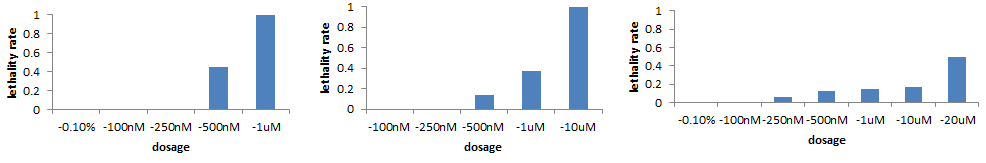
\includegraphics[scale=0.7]{figure/lethalityISV.png}
  \end{center}
  \caption[Effect of varying dosage on ISV]{Lethality rate for three chemicals on ISV. There is an increase in lethality rate with increase in dosage. 0.1\% represents the untreated (control) zebrafish image.}
  \label{lethalISV}
\end{figure}

\begin{figure}[H]\centering
  \begin{center}
    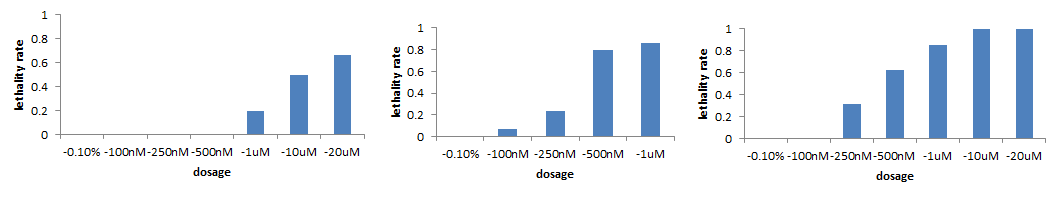
\includegraphics[scale=0.7]{figure/lethalityCVP.png}
  \end{center}
  \caption[Effect of varying dosage on CVP]{Lethality rate for three chemicals on CVP. There is an increase in lethality rate with increase in dosage. 0.1\% represents the untreated (control) zebrafish image.}
  \label{lethalcvp}
\end{figure}
\end{landscape}

Based on lethality rate, we deduced out of 38 screened chemicals, our ISV model identified 28 chemicals that severely ($\geq$ 10\% of embryos are impacted for each dosage within each chemical) impacted ISV growth. Out of 28 chemicals impacting ISV growth, 22 of them showed increasing lethality rate with increasing dosage. Remaining 6 chemicals did not show an increment in lethality rate with increasing dosage, but the effects are more sever at high dosages. Figure \ref{lethalISV} shows lethality rate for three chemicals with increasing dosage. Its worth pointing out that in some cases our model identified untreated zebrafish as unhealthy. Reasons for the miss-classification is due to the imaging artifact. There are 20 images out of 2039, in which zebrafish turned on its back during imaging. We have isolated those images while calculating lethality rate. We can calculate safe dosage as maximum dosage within each chemical with 0 lethality rate.

On similar line as above, we computed lethality rate for CVP analysis. 30 chemicals out of 38 severely ($\geq$ 10\% of embryos are impacted for each dosage within each chemical) impacted development in CVP region. Out of 30 chemicals impacting CVP, 15 showed increasing impacts on CVP with increasing dosage (in terms of lethality rate). Figure \ref{lethalcvp} shows lethality rate for three chemicals with increasing dosage.



\begin{figure}[H]\centering
  \begin{center}
    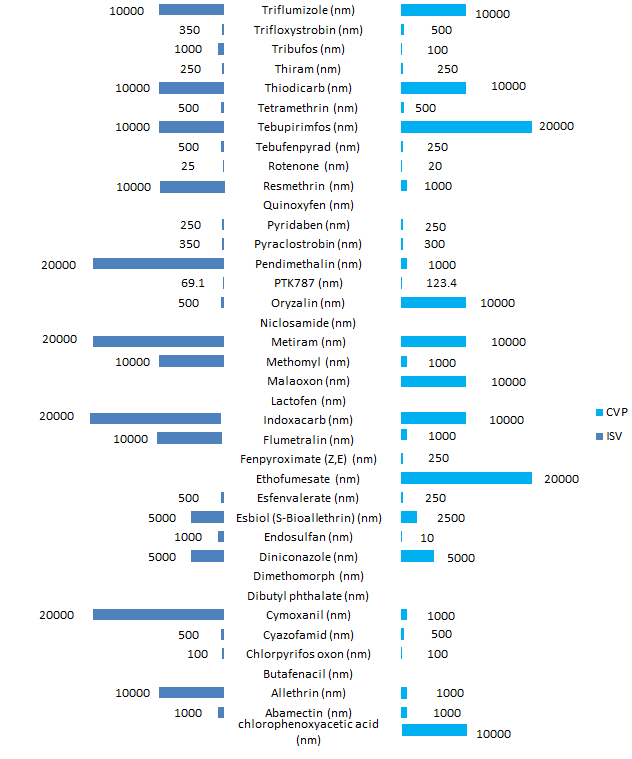
\includegraphics[scale=0.8]{figure/chemicalProfile.png}
  \end{center}
  \caption[Safe Dosage for ISV and CVP]{Figure tells us chemicals, which impact ISV only, CVP only, both ISV and CVP. Safe dosage for each chemical for ISV and CVP region is also illustrated in this plot. Each dosage is given in nanometer (nm). Chemical with the blank value, shows there is no impact due to toxicity for tested dosages.}
  \label{lethalcvpisv}
\end{figure}

A representation is illustrated to show what is the safe dosage for chemical based on ISV and CVP based screening ( fig.\ref{lethalcvpisv}) . This illustration also tells us which chemicals impacted ISV only, CVP only or both ISV and CVP. Moreover it tells us the safe dosage for various chemicals used to treat zebrafish embryo. For 15 chemicals, we found exactly same safe dosage for both ISV and CVP. In 15, of them difference is one step of dosage. By, one step of dosage we mean, lets say dosages tested are 10nm, 100nm, 250nm for a chemical. ISV and CVP shows 100nm and 250nm as safe dosage respectively. Hence we say dosage difference is one step between ISV and CVP. 4 chemicals had a difference of two steps for safe dosages for ISV and CVP. In remaining 4 the difference is more than two steps.

\section{Vasculature Time - Series Analysis}
The computational framework presented in section \ref{sec:timelapse} is applied to quantify vascular changes in both toxin treated and untreated zebrafish embryos. A uniform B-splines control grid with spacing $[20, 20]$, and 3 grid refinement levels are used. Totally, 7 embryos (5 untreated and 2 treated) are analyzed. Vascular growth is computed using method described in section \ref{sec:timelapse}. Figure \ref{toxicityAvgAs} shows the dynamics of blood vessel growth in terms of average pixel change for untreated and arsenic treated embryos. As seen in the figure, although the overall rate of growth is constant for both treated and untreated embryos, the growth rate for untreated embryos is approximately 5 times higher.  

\begin{figure}[!p]
  \begin{center}
    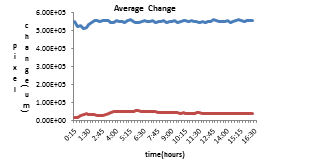
\includegraphics[scale=1]{figure/AvgAs.png}
  \end{center}
  \caption[Average comparison between healthy and treated]{Blue curve shows average change in number of pixels over all the unexposed embryos whereas red curve shows average pixel change for arsenic treated embryo.}
  \label{toxicityAvgAs}
\end{figure}

Figure \ref{toxicityAllAs} shows the dynamics of blood vessel growth in terms of average pixel change for each of the seven embryos analyzed. Pixel change measured in untreated fish is represented by uexposed1 - uexposed5 and exposed1 - exposed2 shows pixel change measured for arsenic exposed embryos.
\begin{figure}[!p]
  \begin{center}
    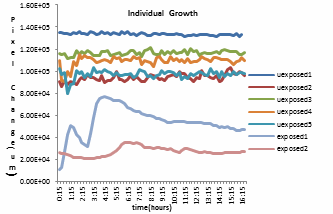
\includegraphics[scale=1]{figure/AllAs.png}
  \end{center}
  \caption[Individual comparison between healthy and treated]{uexposed1 - uexposed5 represents change in number of pixels for unexposed embryos growth, whereas exposed1 and exposed2 represents change in number of pixels for arsenic treated embryos.}
  \label{toxicityAllAs}
\end{figure}
